\documentclass[tikz,border=8pt]{standalone}
\usepackage{tikz}
\usetikzlibrary{positioning,fit,backgrounds,calc,arrows.meta}
\usepackage{xcolor}

\definecolor{ugmblue}{HTML}{194168}
\definecolor{degreen}{RGB}{76,175,80}
\definecolor{dered}{RGB}{229,115,115}

\begin{document}
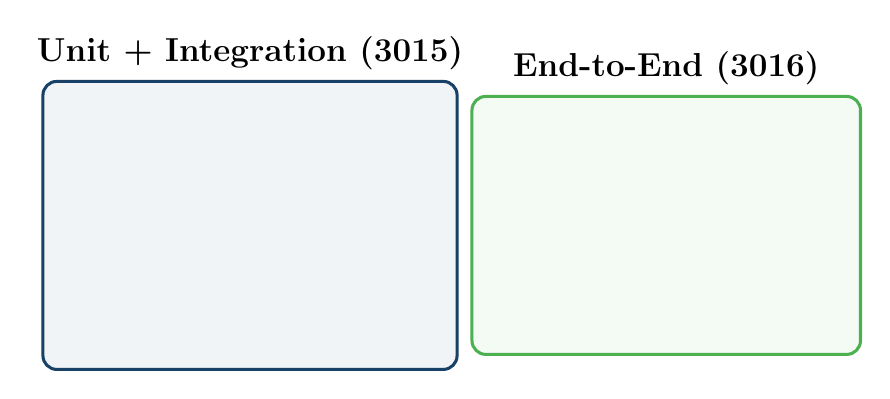
\begin{tikzpicture}[
    node distance=0.4cm and 0.5cm,
    box/.style={rectangle, rounded corners=3pt, draw=#1, fill=#1!8,
                minimum width=2.7cm, minimum height=0.72cm, align=center,
                line width=0.9pt, font=\large},
    group/.style={rectangle, rounded corners=5pt, draw=#1, fill=#1!6,
                  inner sep=6pt, line width=1.1pt},
    lbl/.style={font=\large\bfseries}
]

% Left: Unit + Integration
\node[box=ugmblue] (u1) {FetchEmployeeIssuesTool\\56 unit + 5 integ \textbullet{} 100\%};
\node[box=ugmblue, below=0.3cm of u1] (u2) {SQL-injection test};
\node[box=ugmblue, below=0.3cm of u2] (u3) {drive search 100\%};
\node[group=ugmblue, fit=(u1)(u2)(u3),
      label={[lbl]above:Unit + Integration (3015)}] (unit) {};

% Right: End-to-End
\node[box=degreen, right=1.2cm of u1] (e1) {Playwright MoM};
\node[box=degreen, below=0.3cm of e1] (e2) {Playwright Datasaur};
\node[box=degreen, below=0.3cm of e2] (e3) {consolidated env-driven};
\node[group=degreen, fit=(e1)(e2)(e3),
      label={[lbl]above:End-to-End (3016)}] (e2e) {};

\end{tikzpicture}
\end{document}
